\documentclass[fontsize=12pt,paper=a4]{jlreq}

\usepackage{graphicx}

\title{\LaTeX での図表の配置}
\author{筑波大学 三末和男(改訂:中井央)}
\date{2015年6月2日(2023/04/15 改訂)}

\begin{document}
\maketitle

\section{はじめに}

論文等の文書にはしばしば図表が含まれる。
ここでは、\LaTeX での図表の扱いについて説明する。
図表の配置のための環境の他に、表そのものを作成するための環境がある。
これらを混同しないように注意して欲しい。
\LaTeX は図を描く機能も備えているがあまり便利ではない。
図は別のソフトウェアで作成する方が容易である。

\section{図の配置}

図の配置には figure 環境を使用する。
下のように記述することで図のスペースとして縦方向に 50mm 分確保できる。
キャプション (caption) は図の説明文である。
論文等に図を配置する際には必ずキャプションを付ける。
図のキャプションは図の下に配置するのが慣習である。
\begin{quote}
\begin{verbatim}
\begin{figure}
\vspace{50mm}
\caption{男女別の身長と体重の関係}
\label{fig:bodysize}
\end{figure}
\end{verbatim}
\end{quote}

さて、印刷後に紙を使って切り貼りするのであれば、
これでもよいが実際には空白を空けるのではなく、
図を挿入する。
そのためには\verb|\vspace{50mm}|の代りに下のような行を入れる。
\begin{quote}
\begin{verbatim}
\centering
\includegraphics[width=0.8\hsize]{figure1png.png}
\end{verbatim}
\end{quote}
なお、図を横方向中央に配置するために\verb|\centering|を指定している。

\begin{figure}[h]
\centering
\includegraphics[width=3cm,height=6cm,angle=67]{figure1png.png}
\caption{男女別の身長と体重の関係}
\label{fig:bodysize}
\end{figure}
\begin{figure}[h]
\centering
\includegraphics[width=3cm,height=6cm,angle=67]{figure1png.png}
\caption{男女別の身長と体重の関係}
\label{fig:bodysize}
\end{figure}

この例ではPNGファイルを埋め込んだ。

PNG ファイルは画面のキャプチャや PowerPoint によって手軽に作成できる
\footnote{PowerPoint で作成した図を PNG 形式で保存するには、
図を選択し、右ボタンメニューで「図として保存...」を選べばよい。
いくつかのファイル形式が指定できるが、PNG がデフォルトである。}
ので便利であるが、
ラスターデータであるため拡大するときたなくなる。
拡大してもきれいな図を作成するにはベクター形式 (EPS) で作成する必要がある。
EPS ファイルの図を作成する場合には Illutrator や
LibreOffice などが使用できる。

\begin{figure}[t]
\centering
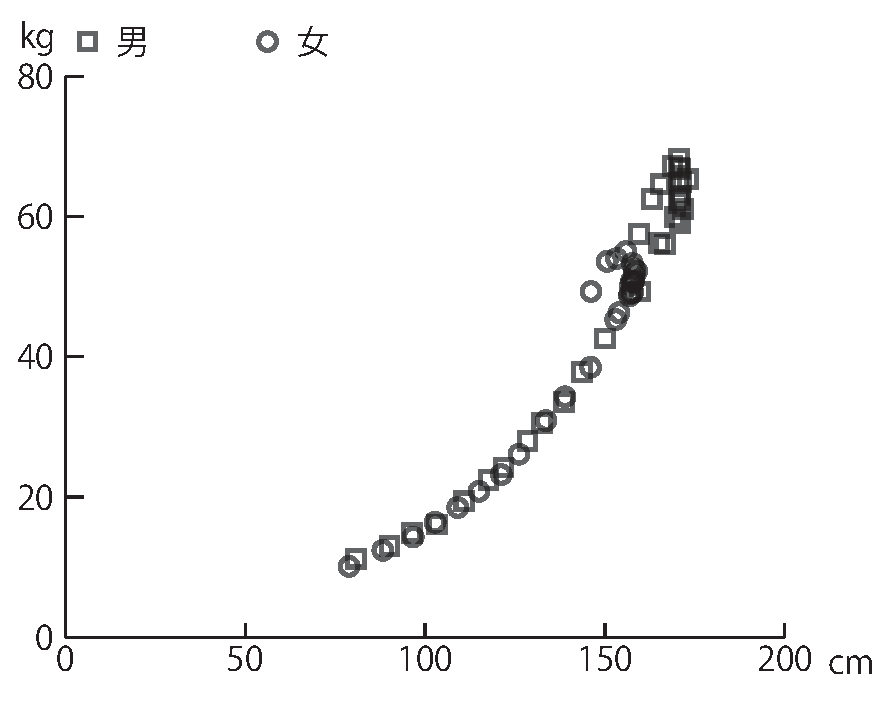
\includegraphics[width=0.8\hsize]{figure1eps.eps}
\caption{男女別の身長と体重の関係(EPS版)}
\label{fig:bodysize2}
\end{figure}

PNG と EPS の違いはこの文書を PDF に変換して、
図\ref{fig:bodysize} と図\ref{fig:bodysize2} を拡大して比較するとよく分る。


\section{表の配置}\label{sec:table}

表の配置には table 環境を使用する。
table 環境の使い方は figure 環境と同じである。
下のように記述することで、表のスペースとして縦方向に50mm分確保できる。
表のキャプション (caption) は図とは違い、表の上に配置するのが慣習である。
\begin{quote}
\begin{verbatim}
\begin{table}
\caption{男女別の身長と体重の関係}
\label{tab:bodysize}
\vspace{50mm} # 実際にはここで表を記述する
\end{table}
\end{verbatim}
\end{quote}


\section{表の作成}

表を作成するには tabular 環境を使用する。
第\ref{sec:table}節で例に挙げた\verb|\vspace|
\verb|{50mm}|の部分を
tabular 環境による記述で置き換えることで、
実際に表が作成され配置される。
tabular 環境だけでも表を作成できるが表番号などが管理されない。

tabular 環境では、
罫線の描き方や表のセル内での配置などさまざまな指定ができる。
いくつかの例を紹介しよう。

\begin{table}[!b]
\caption{男女別の身長と体重の関係}\label{tab:bodysize}
\centering
\begin{tabular}{p{1cm}|p{2cm}|p{3cm}|p{4cm}}
\cline{2-3}
体重(男)& 身長(男)& 体重(女)& 身長(女)\\
\hline
11.2 & 80.8 & 10.1 & 78.9 \\
13.0 & 90.1 & 12.4 & 88.3 \\
14.9 & 96.3 & 14.3 & 96.7 \\
16.1 & 103.4 & 16.4 & 102.8 \\
19.4 & 110.9 & 18.5 & 109.1 \\
\hline
\end{tabular}
\end{table}

横書き文化圏では表\ref{tab:bodysize}のように横罫線だけを使用するのが普通である。

\begin{table}[h]
\caption{男女別の身長と体重の関係}\label{tab:bodysize2}
\centering
\begin{tabular}{|cc|cc|}
\hline
体重(男)& 身長(男)& 体重(女)& 身長(女)\\
\hline
11.2 & 80.8 & 10.1 & 78.9 \\
13.0 & 90.1 & 12.4 & 88.3 \\
14.9 & 96.3 & 14.3 & 96.7 \\
16.1 & 103.4 & 16.4 & 102.8 \\
19.4 & 110.9 & 18.5 & 109.1 \\
\hline
\end{tabular}
\end{table}

日本では縦罫線も多用するので表\ref{tab:bodysize2}のように書くことも多い。表\ref{tab:bodysize2}ではさらに中揃えにしてみた。

\begin{table}[h]
\caption{男女別の身長と体重の関係}\label{tab:bodysize3}
\centering
\begin{tabular}{|r|r||r|r|}
\hline
\multicolumn{2}{|c||}{男} & \multicolumn{2}{c|}{女} \\
体重& 身長& 体重& 身長 \\
\hline
11.2 & 80.8 & 10.1 & 78.9 \\
13.0 & 90.1 & 12.4 & 88.3 \\
14.9 & 96.3 & 14.3 & 96.7 \\
16.1 & 103.4 & 16.4 & 102.8 \\
19.4 & 110.9 & 18.5 & 109.1 \\
\hline
\end{tabular}
\end{table}

部分的に列をまとめたいこともある。たとえば、表\ref{tab:bodysize3}は見出しの「男」、「女」をそれぞれまとめたものである。

\end{document}
